\documentclass[border=4pt]{standalone}
\usepackage{tikz}
\usetikzlibrary{shapes.geometric,positioning,arrows.meta}

\begin{document}
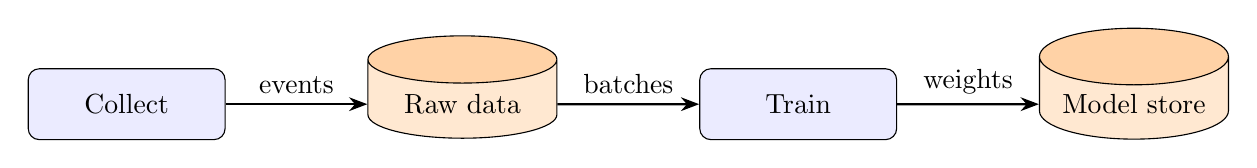
\begin{tikzpicture}[
  >=Stealth,
  node distance=18mm,
  process/.style={draw,rounded corners,minimum width=25mm,minimum height=9mm,fill=blue!8},
  store/.style={cylinder,shape border rotate=90,shape aspect=.35,draw,
    minimum width=24mm,minimum height=13mm,cylinder uses custom fill,
    cylinder body fill=orange!18,cylinder end fill=orange!35},
  flow/.style={->,thick}
]
  \node[process] (collect) {Collect};
  \node[store,right=of collect] (raw) {Raw data};
  \node[process,right=of raw] (train) {Train};
  \node[store,right=of train] (model) {Model store};

  \draw[flow] (collect) -- node[above]{events} (raw);
  \draw[flow] (raw) -- node[above]{batches} (train);
  \draw[flow] (train) -- node[above]{weights} (model);
\end{tikzpicture}
\end{document}
